\chapter{Introduction}
Each year, many thousands of trucks are involved in traffic accidents; in 2008, 380,000 trucks were involved in accidents \cite{NHTSA2008}.
Litigation connected with these crashes can result in judgments in the millions of dollars. In recent years, this litigation has 
come to depend more and more heavily on electronic event data recorded on the trucks' engine control systems. 
This evidence includes speed records and other event data that can help accident reconstructionists 
determine what transpired during the event.

Like other evidence, heavy vehicle digital event data is held to a standard of forensic soundness, which is a series of principles 
that ensure that forensic evidence is handled in a secure manner that guards against misinterpretation and alteration, whether intentional
or unintentional.
Currently, evidence is extracted from heavy truck systems using software that was not originally designed to be 
forensic software, and is not particularly suited to the task. While evidence can be collected using this data in a forensically sound 
manner, doing so requires diligence on the part of the investigator and mistakes can result in evidence being dismissed. Additionally, 
the current methods by which data are stored are not particularly resistant to tampering. 

\section{Truck ECMs and Evidence}

Beginning in the early 1990s, truck engine manufacturers implemented electronic engine control in order to meet more stringent emissions
requirements placed on large diesel vehicles. Over time, demand from fleet customers lead to implementation of data logging within these
engine control computers, including fuel usage tracking and driver behavior . NHTSA then requested the engine manufacturers to investigate the implementation
of event data recorder (EDR) functionality in heavy truck ECMs. Shortly thereafter, manufacturers began offering this functionality in their
ECMs, first as add-on packages then as standard features.

The evidence contained within the heavy truck ECMs is extracted using diagnostic software provided by the manufacturer. Some popular
manufacturers and the associated software of forensic interest is listed in Table \ref{tab:software}.

\begin{table}
\centering
\begin{tabular}{|l|l|}
\hline
\emph{ECM Family} & \emph{Software}\\
\hline
Caterpillar & Caterpillar Electronic Technician (CatET)\\
\hline
Cummins & Cummins PowerSpec, Cummins Insite\\
\hline
Detroit Diesel & DDEC Reports, Detroit Diesel Diagnostic Link (DDDL)\\
\hline
Mack & Proprietary to Mack and Volvo\\
\hline
Mercedes & DDEC Reports, Detroit Diesel Diagnostic Link (DDDL)\\
\hline
Navistar & ServiceMaxx \\
\hline
Paccar & Cummins PowerSpec, Cummins Insite, or Paccar Davie\\
\hline
Volvo & Mack and Volvo Proprietary\\
\hline
\end{tabular}
\caption{ECMs and associated software}
\label{tab:software}
\end{table}
While it may be tempting to trust the interpretation of the OEM software, research has shown 
that the interpretation of the data may be an issue. For example, in some Cummins Sudden Deceleration 
events, speed data is reported in the report at one sample per second; however, after comparing to 
external reference measurements, it is discovered that the data actually is reported at 0.2 second 
intervals (5 Hz)\cite{bortolin2009}. Similarly, Austin and Farrell \cite{austin2011} showed that many Snapshot records 
from Caterpillar are reported every 0.5 seconds instead of every second as represented in the OEM software.

\section{Heavy Vehicle Networks}

In modern automobiles, the number of in-vehicle electronic devices that need to communicate with one another is increasing rapidly:
engine control modules, anti-lock brake system modules, transmission control modules, collision detection systems, and even entertainment systems are examples of
devices that need to communicate. This lead to a combinatorial explosion of communication links, necessitating a common multiple-access
bus. Now, almost all functions in automobiles are carried out over the network. Notably, in-vehicle networking has allowed external diagnostic
connectors to receive diagnostic fault codes through a port in the cab.

Heavy trucks are no different. Engine control computers monitor vehicle speed and enforce pre-set speed limits. They also broadcast information
for other modules to use; for example, speedometer and tachometer displays on the instrument panel display information received from the vehicle
network. Telematics systems monitor vehicle performance and behavior using the same data. Additionally, vehicle diagnostic communications use
this network. As crash evidence is extracted using diagnostic programs, vehicle networks are of interest to anyone interested in extracting
crash information. There are two major vehicle network standards used in heavy trucks, SAE J1708/1587\cite{J1708}\cite{J1587} and SAE J1939\cite{J1939-71}.

\subsection{SAE J1708/SAE 1587}

SAE J1708 is the older of the two major standards, having been adopted in 1986. It defines the physical layer of the network,
with the higher layers handled by the J1587 standard. It is based upon the RS-485 standard for serial communication, converted to 
unipolar drive. A J1708 message has a fairly straightforward format. The first byte is the Message Identification character
, or MID, which identifies the originator of the message. A number of data bytes, followed by a checksum byte, follows. If the vehicle is running, 
the total length of the data and checksum should not exceed 21 bytes\cite{J1708}. However, there is no upper bound on message size if the vehicle 
is not running. The checksum is calculated by taking the two's complement of the sum of the data bytes.

Individual data elements and their meanings are governed by the J1587 standard\cite{J1587}. This includes specific codes for individual data items,
Parameter Identification characters (PIDs), and the formats for the data to which those PIDs refer. In addition to standardized definitions, 
the J1587 standard also allows for proprietary messages that are designed by individual manufacturers; those proprietary messages are frequently used by 
diagnostic programs.

\subsubsection{Transport Layer}

Standard J1708/J1587 messages are limited to 21 bytes when the engine is not running; in practice, messages longer than this are rare even if the engine
is not running. To allow for the transmission of longer messages, J1587 defines a transport layer that ensures in-order delivery and reliable delivery.

The J1587 transport layer is implemented using two PIDs, 0xC5 and 0xC6. PID 0xC5 is defined as the connection management PID, implementing traffic control
functions. PID 0xC6 is the data transfer PID, which is used to transfer data. The node that wishes to send a transport message first sends a Request To Send
(RTS) message indicating the total size of the message, as well as the number of segments that will be sent. The recipient node will then respond with a 
Clear To Send (CTS) message indicating the next segment number expected and the number of frames the recipient can accept. The sender then replies with
the appropriate number of frames, each with PID 0xC6 and containing a sequence number. The recipient uses CTS messages to indicate to the sender that
more frames can be sent, and also to request the retransmission of lost frames.

When the recipient has received the number of messages indicated in the RTS message, it sends an EOM message. At any time, if a node needs to abort the
connection, an ABORT frame is sent. The standard mandates a 60 second wait before timing out a connection.

\subsubsection{Proprietary PID}

The format of a proprietary message is detailed in <INSERT FIGURE HERE>. The first byte is the sender's MID, the second byte is the
proprietary extension PID (0xFE), and the third byte is the recipient's MID. Any data in the frame thereafter is defined by the manufacturer.

\subsection{SAE J1939}

SAE J1939\cite{J1939-71} is the newer standard, adopted in the year 2000. The physical layer is based on the CAN bus standard developed by Bosch, which is widely in use
in passenger vehicles as well as industrial control applications. The CAN bus standard provides many improvements over the J1708 physical layer,
including more advanced error-checking using CRCs instead of a simple checksum and improved access control on the bus. Unlike the CAN bus commonly used in
passenger vehicles, the J1939 standard uses a 250K baud CAN connection.

The J1939 standard is divided into many documents, as it is much broader in scope than its predecessors. It not only describes standardized
message formats for vehicle bus information, but also specifies a transport-layer protocol for transmitting long messages, protocols for
direct memory access for diagnostic purposes, and more. Like the J1708/J1587 standards, it also allows for proprietary messages unique
to the manufacturer. As with J1708, diagnostic software makes heavy use of proprietary communication protocols.

\section{Diagnostic Link Connector Hardware and Software}

Engine control modules communicate over vehicle-specific networks, so diagnostic software requires a device that can mediate between
vehicle networks and interfaces on desktop computers, such as RS-232 or USB. Those devices are known as Diagnostic Link Connectors, or DLCs.
They connect to a computer via a common interface and translate data to and from J1708, J1939, CAN, and other standards. During normal
operation, a DLC is connected to the in-vehicle network via a diagnostic port in the cab, either a 6-pin or 9-pin Deutsch connector.

The standardization of heavy truck communication has allowed for enhanced interoperation between different brands of products, and DLC
standardization is no different. All DLC manufacturers' drivers must comply with an interface standard dictated by the American Trucking Association's (ATA)
Technical Maintenance Council (TMC), known as TMC RP1210\cite{RP1210}. The RP1210 interface specifies a number of functions that compliant drivers must export,
including function names and formats for arguments. This allows a diagnostic program to utilize any device from any manufacturer. A diagram of the relationship between
the RP1210 interface, the drivers, and device itself is given in figure \ref{fig:rp1210}.

\begin{figure}[h]
  \centering
  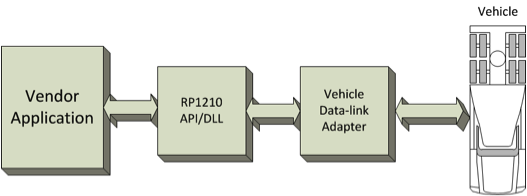
\includegraphics{RP1210}
  \caption{Diagram of RP1210 device and driver}
  \label{fig:rp1210}
\end{figure}

\subsection{RP1210 Functions and Their Uses}

A typical RP1210 session commences as follows. First, the file ``RP121032.INI'' is read to determine which RP1210-compliant devices are installed
on the system. When a device is chosen by the user, the appropriate DLL is loaded into memory and its exported functions are loaded into memory.
As the functions' names and prototypes are standardized, this process is vendor-agnostic.

Next, the client application calls the function \texttt{RP1210\_ClientConnect} to connect to the diagnostic link connector hardware. Assuming
the connection is successful, the client then issues one or more commands using the \texttt{RP1210\_SendCommand} function. This can filter incoming
messages based on MID or PGN, claim an address on a J1939 network, and other connection management functions. After the message filtering has been
set up, the client then uses \texttt{RP1210\_SendMessage} and \texttt{RP1210\_ReadMessage} to communicate on the network. The client terminates
the session with the \texttt{RP1210\_ClientDisconnect} call.

\section{Current Practices}

With the hardware and software requirements established, the typical procedure for an information download from heavy trucks can now be explained.
As mentioned previously, the information is typically downloaded using the engine manufacturer's diagnostic software. The normal use case
for diagnostic software is connecting to a diagnostic port in the cab of the truck using a diagnostic link connector, and accessing the desired
information with the maintenance software.

However, extracting crash information is not a normal use case. Because the truck has been in a high speed collision, the electrical connection
between the cab and the engine may have been severed, or the cab itself may be physically inaccessable. In these cases, the engine control module
must be removed and analyzed separately. This is performed either by placing the ECM in a donor vehicle identical to the one in the crash, or
by connecting to the ECM directly using the manufacturer's engine flashing harness. A bench download of a Cummins ECM is shown in figure \ref{fig:cumminsbench}.

Whatever method was used to connect to the ECM, the investigator then proceeds to extract the information using the manufacturer's diagnostic
software. This includes event data from the crash itself, mechanical fault information, engine tuning parameters, and driver behavior information.
This information is then recorded, in most cases, by printing the data to a PDF file. However, in many instances the software does not support
printing data and so it must be captured using a screenshot. All of the files resulting from the extraction are then stored on some kind of
removable media and produced to the client.

\subsection{For Contrast: Hard Disk Forensics}

In order to put current evidence handling practices for ECMs in the context of digital forensics in general, here the evidence extraction
procedures for hard disk drives is briefly explained. A more thorough treatment of this subject is given in \cite{carrier2005}.

Evidence disk drives are typically \emph{imaged}; that is, data is copied off the drive in the most raw form available from outside
the drive itself. The image is nothing more than a string of bits that have been copied sequentially from the disk drive. It includes
partition tables, filesystem metadata, deleted files, and more.

Devices called \emph{write blockers} are used to ensure the integrity of the evidence drive. They mediate the connection between the
drive and the computer that is imaging it, and any write commands originating from the computer are not forwarded on to the drive.
This prevents any accidental writes caused by investigator mistakes, automatic attempts by operating systems to mount file systems, etc.
Furthermore, the original disk is rarely accessed after the initial extraction, as all subsequent analysis is performed on the image.

To detect tampering or data corruption, the disk image is fingerprinted using a cryptographic hash function. This fingerprint is then recorded,
and can be verified later by re-hashing the image. Assuming that the hash itself can be protected, this re-hashing allows investigators to
detect any changes in the data.

\begin{figure}[h]

  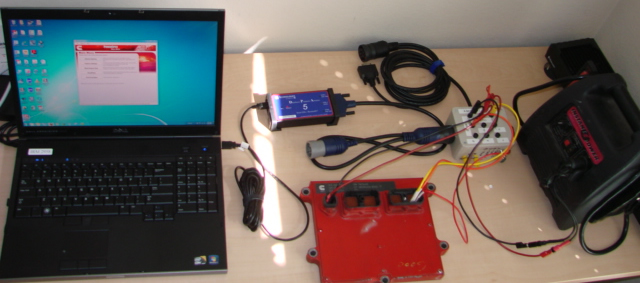
\includegraphics[scale=0.5]{cumminsbench}
  \caption{A bench download from a Cummins ECM}
  \label{fig:cumminsbench}
\end{figure}

\section{Forensic Soundness}

A heavy vehicle electronic control module (ECM) is a specialized process control computer that may have data of interest to an investigator. 
While ECMs may not have keyboards and monitors, they still are computers and have central processing units, memory, storage, and a means of 
networking or communicating with external devices. As such, many of the principles from computer forensics can be applied to heavy vehicle ECMs.

The first litmus test that any forensic methodology must pass is the rules of evidence for the legal system in which it is used. Here, we will
focus on the laws of the United States. The two primary standards to which evidence is held in that country are the Daubert standard, established
in the case \emph{Daubert v Merrell Dow Pharmaceuticals}, and the Federal Rules of Evidence. A review of the rules of evidence as they relate to 
digital forensics may be found in \cite{meyers2005}.

\begin{enumerate}
  \item Testimony must be relevant and reliable
  \item Judges have the task of ensuring that expert testimony rests on a reliable
        foundation and is relevant.
  \item Some or all of certain specific factors, including testing, peer review, error
        rates, and acceptibility in the relevant scientific community, may prove helpful
        in determining reliability of forensic testimony.
\end{enumerate}

\begin{enumerate}
  \item Method can be and has been tested
  \item Method has been subjected to peer review or publication.
  \item Method has a known error rate
\end{enumerate}

In addition to the general rules of evidence, the digital forensics literature contains many attempts to quantify the concept of forensic soundness.
A Special Report issued by the National Institute for Justice on Electronic Crime Scene Investigation \cite{NIJ2008} highlights the following basic forensic 
principles applied to dealing with digital evidence:

\begin{itemize}
\item Any process or procedure of collecting, transporting, or storing of digital evidence should not incur any changes to the evidence.
\item Only specifically trained experts should examine digital evidence.
\item Transparency during the operations of acquisition, transportation, and storage of the evidence should be maintained.
\end{itemize}

These basic tenets lay the foundation for the idea of forensic soundness. It is important to understand the term “forensically sound” 
as it relates to digital evidence. Many authors and professional organizations have attempted to rigorously define this concept, 
including the National Institute for Standards and Technology (NIST) \cite{NIST2001}, law enforcement entities such as the National Institute for 
Justice (NIJ) \cite{NIJ2008}, and academic bodies like the International Organization on Computer Evidence\cite{IOCE2002}. The methods of extracting, analyzing, 
and presenting digital evidence are forensically sound if they perform the task in a manner such that the results can be used in legal 
proceedings with a high degree of confidence in their admissibility. The process of extracting, interpreting, and presenting evidence 
will be referred to in this paper as the “forensic process.”

In addition to the NIJ report, McKemmish \cite{mckemmish2008} enumerates the following components of forensic soundness:

\begin{itemize}
\item \emph{Meaning} is a term that denotes confidence in the interpretation of extracted evidence data.
\item \emph{Error Detection} denotes processes for detecting or predicting errors in the forensic process.
\item \emph{Transparency} means the forensic process is documented, known, and verifiable.
\item \emph{Expertise} is required for those investigators examining digital data.
\end{itemize}

Casey \cite{casey2002} defines 7 levels of certainty for digital evidence that dictate how much weight should be given to the evidence in a case:

\begin{itemize}
\item C0: Evidence contradicts known facts
\item C1: Evidence is highly questionable.
\item C2: Only one source of evidence that is not protected against tampering
\item C3: Source(s) of evidence are more difficult to tamper with but there is insufficient evidence for a firm conclusion, or unexplained inconsistencies exist in available evidence
\item C4: Sole source evidence is protected against tampering or multiple, independent sources of evidence agree but the independent evidence is unprotected from tampering.
\item C5: Agreement of evidence from multiple, independent sources protected from tampering, but small uncertainties exist.
\item C6: The evidence is tamper proof and unquestionable.
\end{itemize}

While many of these levels include requirements that are encompassed by the requirements of error detection and certainty of meaning 
specified by McKemmish, this standard includes the principle of tamper resistance. In addition to protecting the evidence from tampering, 
we submit that a system which can demonstrate the absence of tampering also fulfills this requirement.

\section{Shortcomings of Current Practices}

Though several authors describe the concept of forensic soundness slightly differently, the basic concepts remain the same. The evidence must be extracted in a transparent,
repeatable, and verifiable manner that alters or destroys as little data as possible. There must be a high degree of certainty that the data is interpreted correctly. There must
be measures taken to ensure that the evidence has not been tampered with.

Unfortunately, current practices fail to meet these standards in several respects. First and foremost is that evidence extractions cannot be relied upon to leave the data unaltered.
Some engine maintainance software, by default, clears diagnostic fault codes after they are extracted from the engine. While this is desireable behavior for the software's typical
use case, in a forensic context it is unacceptable. In addition, if a bench download is being performed, the ECM is disconnected from all of the various sytems it was designed to monitor,
causing spurious fault codes to be created. With some manufacturers' products, especially Caterpillar, these can overwrite legitimate fault codes. The damage is made worse when
repeated downloads are conducted.

In addition to data extraction, current practices lack in the forensic soundness of the storage of data as well. No measures are taken to ensure that data have not been tampered
with. Data export formats, typically plaintext HTML or PDF documents, can easily be altered with readily-available software. Some manufacturers' native file formats are encrypted
somewhat, though not strongly: Cummins' EIF format is simply a password-protected ZIP archive, while Detroit Diesel's Drumroll files are encrypted using a simple XOR cipher.
Once decrypted, these files can be altered to remove evidence and re-encrypted easily.

Due to the potential for destruction of the source evidence and alteration of extracted data, it appears that current practice fails to pass the litmus test of forensic soundness
as currently accepted in the digital forensics community.

\chapter{Requirements of a Solution}

Regardless of the meaning of the digital data, it is necessary to present data in its final form in such a way that is transparent of its handling to establish trustworthiness. 
According to the transparency principle of forensic soundness, actions taken by an investigator should be available for later examination. Additionally, any error conditions 
encountered by the software should be recorded so that the legal weight of the evidence may be accurately considered. Audit trails are log files generated by forensic software 
to meet these requirements, and should at least be an option in any forensic solution.

\section{Baseline of Trust}

In order to make a full accounting of potential sources of error in any forensic process, it is important to examine the assumptions that the process requires. Standard methods of 
truck evidence extraction assume that the ECM is reporting data faithfully, that the vehicle network is accurately transmitting the communication to and from the ECM. It also assumes 
the Vehicle Diagnostic Adapter (VDA) is faithfully sending data from the vehicle network to the RP1210 library that is called by the OEM software.

While verifying the correct internal functioning of heavy truck ECMs is beyond the scope of this paper, the fidelity of data transmitted across the various networks (CAN bus, serial 
bus and USB) can be easily verified. Both protocols make use of error-correcting codes that detect transmission errors with very high reliability; for example, the CAN 
Cyclic Redundancy Check that is defined in the CAN standard process and detects all errors from 1 to 5 bits in the data frame, and only fails to detect 0.00018\% of 6-bit 
errors in a CAN frame\cite{koopman2004}. The represents a level of certainty that would take many years to experimentally verify because the likelihood of having an error and not knowing 
it is so low.

\section{Protocols}

Because typical ECM data extractions occur over vehicle networks, analysis of their forensic soundness requires knowledge of the protocols used for communication over those networks.

In heavy trucks, the networking protocols enumerate and define the various data that are transmitted over the in-vehicle network, which in turn provides clues as to the nature 
of the data present in the ECM. For example, a data type that is rounded to the nearest power of ten (186 rounded to 190, for example) when transmitted on the network might 
indicate that the value stored to and reported by the ECM is rounded in a similar fashion.

\section{Authentication}

A cryptographic hash function is an algorithm that generates a “fingerprint” of a given input. This fingerprint is generated in such a way that if a single bit of the input changes, 
roughly half the bits in the output file are altered\cite{schneier1996}. As such, they are commonly used to confirm that data have not been altered. A forensically sound tool should use a hash of 
the extracted truck evidence data to ensure that it has not been altered.

\section{Evidence Preservation}

Ideally, a forensic solution would allow the evidence to be preserved indefinitely. While hard disks are fairly inert when not used, heavy truck ECMs are actual computers that 
have some volatile data elements. One example is the ECM's system clock.

Some of the data on heavy truck ECMs is volatile, meaning that it requires a continuous supply of electrical power to avoid being deleted. One important example is the on-board 
system clock, which is important to investigators because it correlates with the timestamps associated with incident records. An exemplar circuit, shown in figure \ref{fig:clockbatt},is based around 
the EM Micro V3020, as used in several Detroit Diesel ECMs.  It is important that the actual on-board system clock be preserved, because the system clock is not necessarily synched 
up with standard times and the offset from the standard time must be recorded at the time of investigation.

Though the batteries in ECMs are large, and power drains slowly over time, this is an example of potentially critical information that can be lost if not extracted and preserved.

\begin{figure}[h]
  \centering
  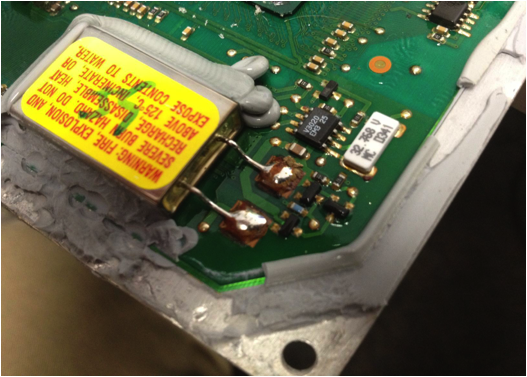
\includegraphics{clockbatt}
  \caption{The real time clock of a Detroit Diesel engine controller with system battery}
  \label{fig:clockbatt}

\end{figure}
